\documentclass[]{report}

\usepackage[portuguese]{babel}
\usepackage[utf8]{inputenc}
\usepackage{graphicx}
\usepackage{hyperref}
\usepackage{mdwlist}
\usepackage{pslatex}
\usepackage{makeidx}
\usepackage{textcomp}
\usepackage{float}
\usepackage{amsmath}
\setlength{\oddsidemargin}{0pt}
\setlength{\evensidemargin}{0pt}
\setlength{\textwidth}{15cm}

% Title Page
\title{}

\makeindex
\begin{document}
\begin{titlepage}
\begin{center}

\textsc{\LARGE Universidade Federal de Santa Maria}\\[1.5cm]
\textsc{\Large Centro de Tecnologia}\\[0.5cm]
\textsc{\Large Departamento de Eletrônica e Computação}\\[0.5cm]
\textsc{\Large Disciplina: Princípios de Telecomunicações}\\[0.5cm]
\setlength{\oddsidemargin}{0pt} % Tirar as margens gigantes que o LaTeX põe
\setlength{\evensidemargin}{0pt} % evitar desperdício de papel
\setlength{\textwidth}{15cm}
\end{center}

\vspace*{5cm}
\begin{center}
{\huge \bfseries Estudo sobre Modulação de Sinais}\\[0.4cm]
\end{center}

\vspace*{130px}
\begin{flushright}
\emph{Autores:}
Caio S. Guedes $<$\url{caio_ee@hotmail.com}$>$ \newline
Marcelo Brum $<$\url{marcelobrum.rs@gmail.com}$>$ \newline
Renan Pinheiro $<$\url{renan.ee.ufsm@gmail.com}$>$. \newline



\end{flushright}
\begin{center}
Santa Maria, \today.

\end{center}


\end{titlepage}
\tableofcontents

\chapter{Introdução}

Em telecomunicações, modulação é a modificação de uma onda eletromagnética, para que informação seja transportada por meio de uma onda portadora. Normalmente seu objetivo é facilitar a comunicação através da redução do tamanho das antenas de receptor e transmissor, ou permitir a transmissão de dados por meio de diferentes canais.

Neste trabalho serão abordadas as práticas feitas em laboratório, na disciplina de Princípios de Telecomunicações, visando estudar o funcionamento das modulações em amplitude (AM) e em frequência (FM). Também será abordada, de forma teórica, a modulação por códigos de pulso (PCM). 

\chapter{Aula prática 1: Modulação AM a diodo}
\section{Fundamentação Teórica}
Para ambas as modulações, sejam:

\begin{itemize}
\item um sinal senoidal modulante dado por 

\begin{equation}\label{eq_modulante}
v_s = A_s \cos(\omega_s t)
\end{equation}

\item uma portadora dada por

\begin{equation}\label{eq_portadora}
v_c = A_c \cos(\omega_c t)
\end{equation}
\end{itemize}
tal que $\omega_c > \omega_s$. A fase dos sinais é fixa em $0$, assim eliminando-se $\phi$. 

\subsection{Modulação em Amplitude com Portadora Suprimida (AM-DSB-SC)}
Nos domínios do tempo e da frequência ela é dada por

\begin{equation}\label{eq_am_dsb_sc_tempo}
v_m = v_s v_c = A_s A_c \cos(\omega_s t) \cos(\omega_c t)
\end{equation}

o que no domínio da frequência dá
\begin{equation}
\mathcal{F}(V_m)= \frac{A_s A_c \delta(\omega_s - \omega_c) + \delta(\omega_s + \omega_c)}{2}
\end{equation}

representado no gráfico
\begin{figure}[H]
\begin{center}
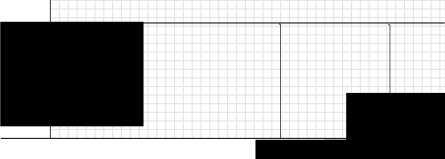
\includegraphics[scale=0.8,clip]{./imagens/frequencia_AM_DSB_SC}
\end{center}
\caption{O sinal AM-DSB-SC no domínio da frequência.}
\label{fig:am_dsb_sc_frequencia}
\end{figure}

O principal problema dessa modulação é que o receptor precisa gerar sua própria portadora para demodulação do sinal. Se ela não estiver sintonizada na exata frequência da portadora original, tem-se a distorção do sinal demodulado. 

\subsection{Modulação em Amplitude com Portadora (AM-DSB)}
Nesta modulação, transmite-se a portadora juntamente ao sinal, simplificando a demodulação. Então a modulação pode ser escrita como
\begin{equation}\label{eq_am_dsb_tempo}
v_m = \underbrace{v_s v_c}_{AM-DSB-SC} + \underbrace{v_c}_{portadora\ adicional} = v_c [1 + v_s]
\end{equation}

e assim no domínio da frequência tem-se que o espectro deste sinal é dado por

\begin{equation}
\mathcal{F}(V_m)= \frac{A_s A_c \delta(\omega_s - \omega_c) + \delta(\omega_s + \omega_c) + A_c \delta(\omega_c)}{2}
\end{equation}

\begin{figure}[H]
\begin{center}
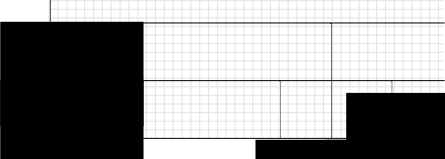
\includegraphics[scale=0.8,clip]{./imagens/frequencia_AM_DSB}
\end{center}
\caption{O sinal AM-DSB no domínio da frequência.}
\label{fig:am_dsb_frequencia}
\end{figure}

Dessa forma, perde-se eficiência mas a demodulação se torna mais simples, como será visto no decorrer deste capítulo.

\section{Procedimento experimental}

Problema proposto:
\begin{quote}
Implemente o circuito da Figura 1 e calcule a frequência de ressonância do filtro passa faixa. Ajuste a frequência de $E_o(t)$ para o valor calculado. Ajuste a frequência de $a(t)$ para 1KHz. Faça a amplitude de $E_0(t)$ igual a 10V pico a pico e a de $a(t)$ 3V pico a pico. Apresente suas conclusões a respeito do uso do filtro e da frequência de ressonância obtida.
\end{quote}


O circuito da figura \ref{fig:demodulador_AM_diodo} foi montado em uma \textit{protoboard}:
\begin{figure}[H]
\begin{center}
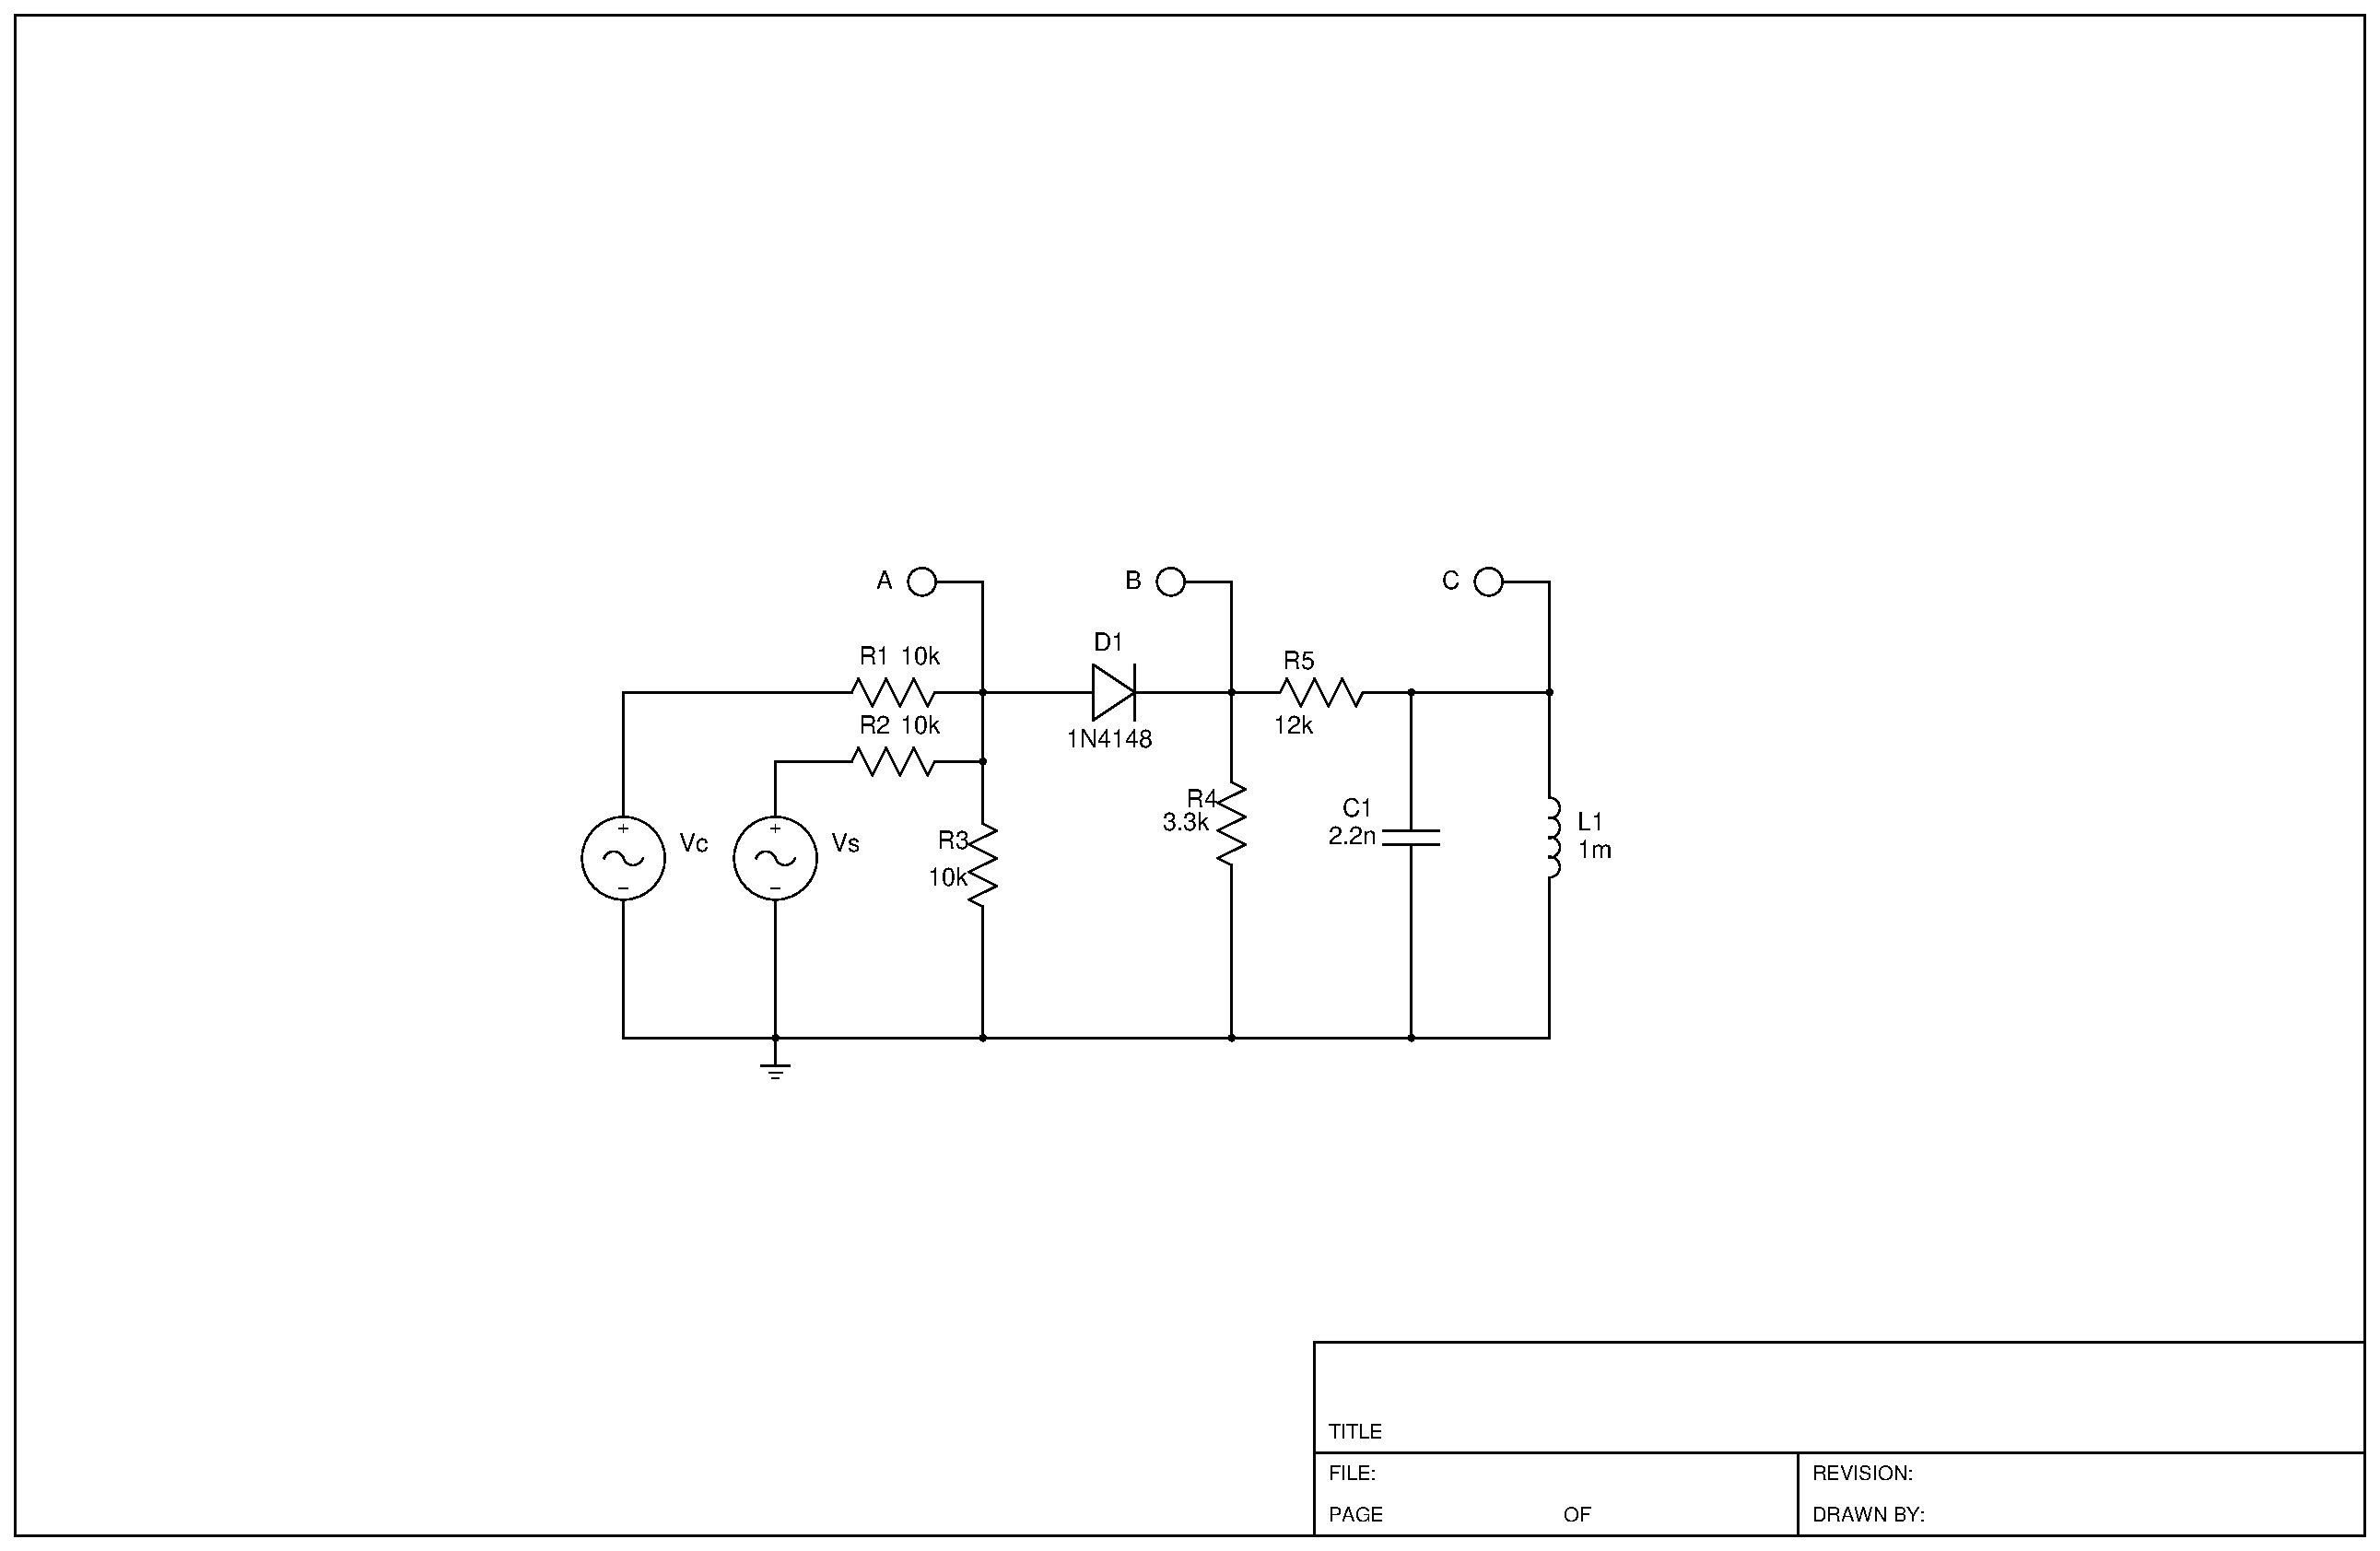
\includegraphics[scale=0.4,clip]{./imagens/AM_Modulator_Diode}
\end{center}
\caption{Modulador AM a diodo.}
\label{fig:demodulador_AM_diodo}
\end{figure}

Para sintonizar a portadora, calcula-se a frequência de ressonância do filtro LC da saída:

\begin{equation}
f_0 = \frac{1}{2 \pi \sqrt{LC}}
\end{equation}

Para os valores fornecidos ($C = 2,2 nF$ e $L = 1000 \mu F$) ter-se-á que essa frequência será de cerca de 107 KHz. 

Após sintonizados os sinais de portadora e da modulante, na saída (ponto C) constata-se a modulação do sinal. Neste contexto, o indutor e o capacitor agem no sentido de limitar a faixa de frequência do sinal modulado.

\section{Resultados}
Disto se determinam:
\begin{itemize}
\item{\bf Frequências dos sinais portador e modulante:} 107 KHz e 1 KHz, respectivamente.

\item{\bf Forma de onda:}
\begin{figure}[H]
\begin{center}
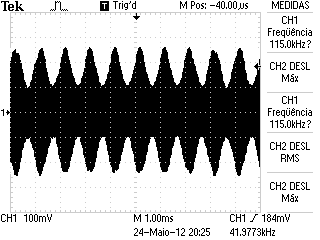
\includegraphics[scale=0.65]{./imagens/AM_Dominio_Tempo}
\end{center}
\caption{Sinal à saída do modulador (ponto \textit{C} no esquemático).}
\label{fig:onda_AM}
\end{figure}
\begin{figure}[H]
\begin{center}
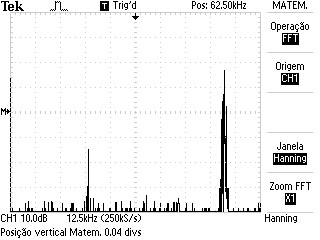
\includegraphics[scale=0.65]{./imagens/AM_Dominio_Frequencia}
\end{center}
\caption{Espectro de frequência deste sinal.}
\label{fig:frequencia_AM}
\end{figure}

Pelo espectro verifica-se que a modulação é do tipo \textbf{AM-DSB}.
\item{\bf Índice de modulação:}
O índice de modulação ($IM$), para um sinal puramente senoidal, é calculado por

\begin{equation}\label{indice_modulacao}
I_m = \frac{M_{max} - M_{min}}{M_{max} + M_{min}}
\end{equation}

Do gráfico \ref{fig:onda_AM} mede-se aproximadamente $M_{min}$ = 100 $mV$ e $M_{max}$ = 240 $mV$; colocando-se esses valores na equação \ref{indice_modulacao} tem-se que $I_m \approx 41,17 \%$.
\item{\bf Potência média do sinal:}

A potência média do sinal, assumido que ele esteja ligado à uma carga de 1 $\Omega$, pode ser calculada por

\begin{equation}
P = \frac{{V_m}^2}{R} = \frac{1}{T}\int\limits_{0}^{T}{V_m^2}dt
\end{equation}

Pode-se demonstrar que no nosso caso isso resulta em

\begin{equation}
P = \frac{{V_p}^2}{2}
\end{equation}

Considerando as bandas laterais teremos que

\begin{equation}
P_t = \frac{{E_p}^2}{2} + \frac{{I_m}^2 {E_p}^2}{4}
\end{equation}

O valor de pico do nosso sinal é de cerca de 240 mV; isso equivale a 28,8 $mW$.
\end{itemize}



\subsection{Perdas no espaço livre}

Pergunta:
\begin{flushright}
\textit{Considerando a potência média do sinal e um receptor AM com sensibilidade de -10 dBm, determine a que distância, no espaço livre, o transmissor poderia estar do receptor?}
\end{flushright}

Desconsiderando os obstáculos e o ganho da antena, pode-se determinar as perdas no espaço livre (FSPL - \textit{Free Space Path Loss}) através da equação

\begin{equation}\label{fspl}
FSPL = (\frac{4 \pi d f}{c})^2
\end{equation}

onde:
\begin{itemize}
\item $c$ é a velocidade da luz no vácuo
\item $d$ é a distância do transmissor (em metros)
\item $f$ é a frequência do sinal (em Hz)
\end{itemize}

A sensibilidade mínima do nosso receptor é -10 $dBm$, o que equivale a 100 $\mu W$. Assim, para determinarmos a máxima distância que o nosso receptor pode estar, escrevemos $100 \mu W = FSPL * 28,8 mW$.

Substituindo-se a equação para a FSPL na expressão anterior e resolvendo-se em função de $d$ tem-se que a máxima distância possível é de \textbf{cerca de 14 m}.

\subsection{Amplificador de saída}

Pergunta:

\begin{flushright}
\textit{Projete, para obter um ganho de transmissão acima de 3 dB, um amplificador para o transmissor do experimento. Mostre os cálculos e apresente uma simulação do circuito.}
\end{flushright}

A forma mais simples de projetarmos um amplificador de saída, tendo em vista a baixa frequência do sinal de saída, é utilizando um amplificador operacional (\textit{op-amp}). Foi empregado um \textit{op-amp} TL072, cujo produto ganho-banda ($G_{BW}$) é 3 MHz - adequado aos propósitos deste trabalho.

Na configuração de op-amp inversor, vista na figura, o ganho é dado por $\frac{-R_{f}}{R_{in}}$:

\begin{figure}[H]
\begin{center}
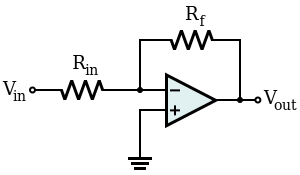
\includegraphics[scale=0.65]{./imagens/Op-Amp_Inverting_Amplifier}
\end{center}
\caption{Amplificador inversor usando op-amp}
\label{fig:opamp}
\end{figure}

Para obtermos o ganho de 3 dB (que equivale aproximadamente a um ganho de 2), emprega-se $R_f$ de 20 $k\Omega$ e $R_{in}$ de 10 $k\Omega$, e para inverter a fase do sinal emprega-se um posterior estágio com ganho 1. Assim obtém-se a saída:

\begin{figure}[H]
\begin{center}
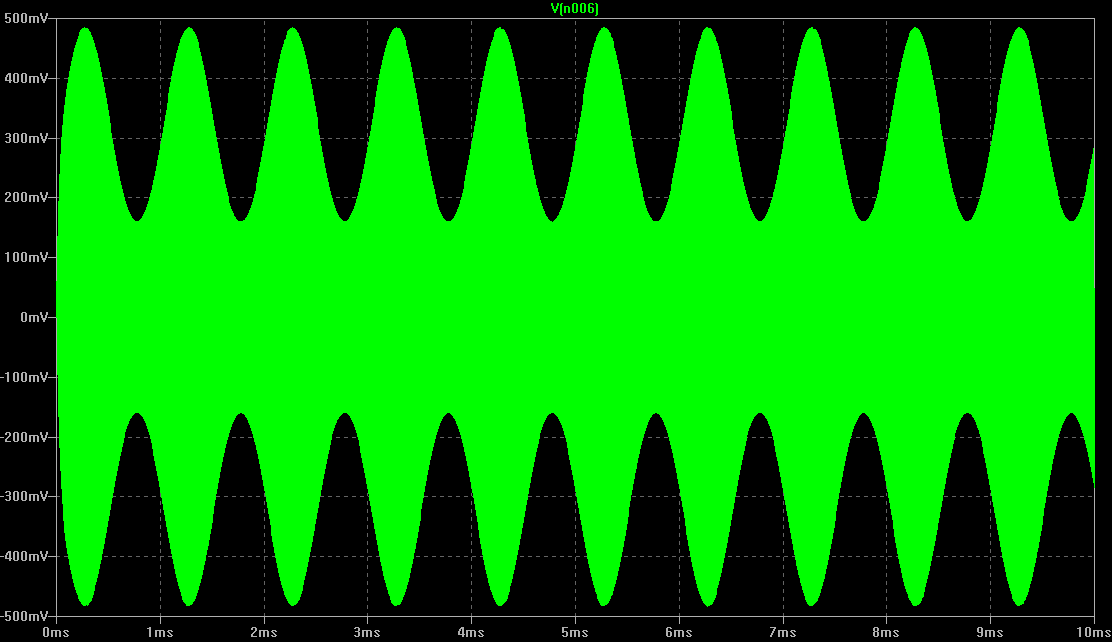
\includegraphics[scale=0.15]{./imagens/sinal}
\end{center}
\caption{Sinal amplificado em 3 dB.}
\label{fig:sinal}
\end{figure}


\subsection{Modulação por diodo}
Pergunta: \begin{flushright}
\textit{Explique como o diodo possibilita a modulação do sinal $E_o (t)$ no circuito implementado na matriz de contatos e apresente o equacionamento que demonstra tal método de modulação.}
\end{flushright}

Suponhamos o diodo como uma chave que permite apenas a passagem da região positiva da onda da portadora. Esse diodo pode ser considerado como um dispositivo não linear, expresso por 

\begin{equation}\label{eq_diodo}
e_1(t) = A \times e_0(t) + bB \times e^2_0(t)
\end{equation}
Ao diodo chega a soma dos sinais da portadora e da modulante: 

\begin{equation}\label{eq_soma_sinais}
e_0(t) = v_s + v_c
\end{equation}

Substituindo \ref{eq_soma_sinais} em \ref{eq_diodo} temos que

\begin{equation}
e_1(t) = k (A (v_c + v_s) + B (v_c + v_s)^2)
\end{equation}

onde $k$ é uma constante, e substituindo \ref{eq_modulante} e \ref{eq_portadora} nessa expressão, ter-se-á que

\begin{equation}
e_1(t) = k(A(A_s \cos(\omega_s t) + A_c \cos(\omega_c t)) + B(A_s \cos(\omega_s t) + A_c \cos(\omega_c t))^2)
\end{equation}

\begin{equation}
e_1(t) = k(A (A_c \cos(\omega_c t) + A_s \cos(\omega_s t) + \frac{b A_c^2 \cos^2(\omega_c t)}{2} + b A_c A_s \cos(\omega_c t - \omega_s t) + \frac{b A_s^2 \cos^2{\omega_s t}}{2}))
\end{equation}

Porém o termo quadrático cria um sinal indesejável na saída, para removê-lo se usa o filtro LC. Então, temos que:

\begin{equation}
e_1(t) = k \{a A cos(\omega_c t) + 2 b A \cos(\omega_s t) \cos(\omega_c t) + \underbrace{a \cos(\omega_c t) + b \cos^2(\omega_c t) + b A^2 [\frac{1}{2} + \frac{cos(2 \omega_c t)}{2}]}_{Filtrado\ pelo\ filtro \ LC}\}
\end{equation}

permanecendo o termo

\begin{equation}
k\{\underbrace{a A cos(\omega_c t)}_{1} + \underbrace{2 b A \cos(\omega_s t) \cos(\omega_c t)}_{2}\}
\end{equation}

constituído pela portadora (1) e pelo sinal modulado (2).


\subsection{Demodulação do sinal}
Pergunta: 
\begin{flushright}
\textit{Simule, considerando os sinais envolvidos no experimento realizado, a demodulação do sinal modulado.}
\end{flushright}
Um demodulador simples, para a transmissão AM-DSB, pode ser implementado através de um circuito detector de envoltória constituído por um diodo e um circuito RC, ajustado para a frequência da modulante. A frequência de corte pode ser calculada através da resposta em frequência do circuito RC, e será de

\begin{equation}
f_c = \frac{1}{2 \pi R C}
\end{equation}

Para a nossa modulante, temos que $R = 5.895 k\Omega$ e $C = 27 nF$ fornecerão uma frequência de corte de  1 KHz. Assim, monta-se o circuito:

\begin{figure}[H]\label{demodulador_AM}
\begin{center}
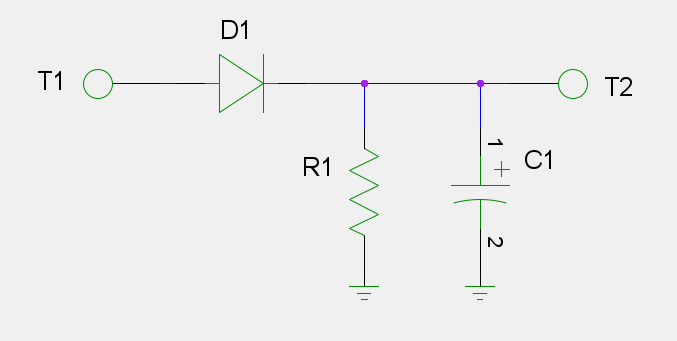
\includegraphics[scale=0.35]{./imagens/Demodulador_AM}
\caption{Demodulador AM. $T_1$ é a entrada do sinal, que sairá demodulado de $T_2$}
\label{fig:demod_AM}
\end{center}
\end{figure}

obtém-se o gráfico:

\begin{figure}[H]
\begin{center}
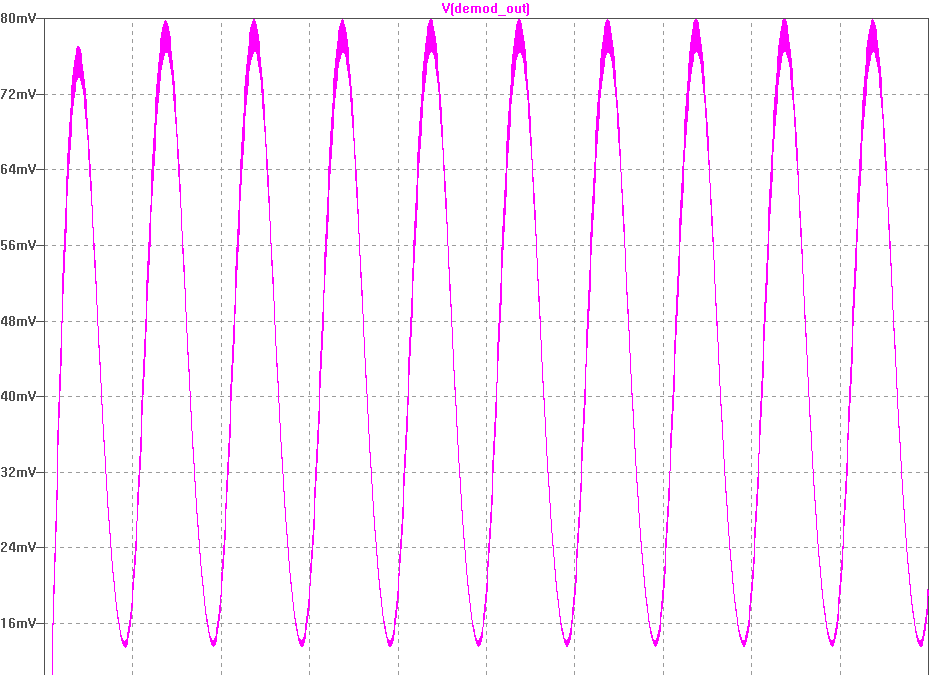
\includegraphics[scale=0.24]{./imagens/grafico_demodulada}
\caption{Sinal demodulado através do circuito da figura \ref{demodulador_AM}}
\label{fig:demodulada}
\end{center}
\end{figure}


\chapter{Aula prática 2: Modulação AM a transistor}

\begin{figure}[H]
\begin{center}
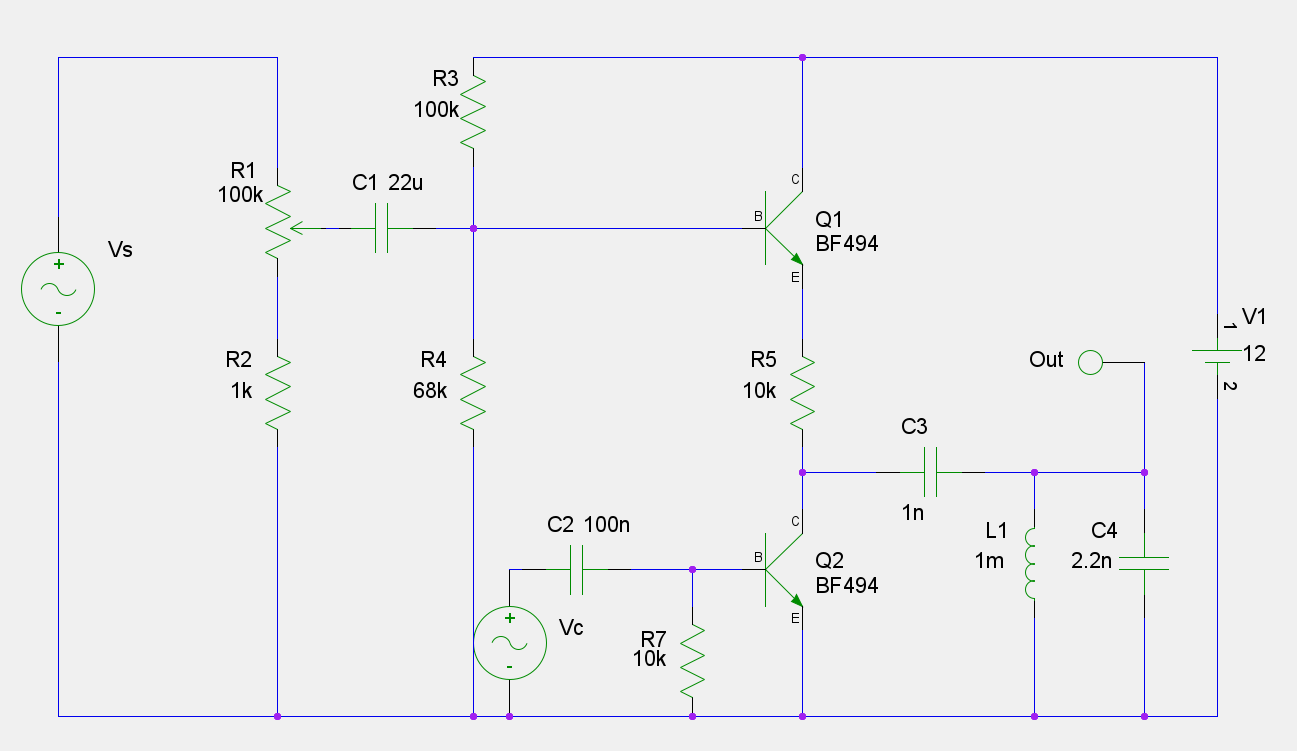
\includegraphics[scale=0.25,clip]{./imagens/AM_Modulator_Transistor.png}
\end{center}
\caption{Modulador AM a transistor.}
\label{fig:modulador_AM_transistor}
\end{figure}

O sinal modulado é gerado utilizando-se os transistores BF494 \cite{BF494}, de alta frequência (até 120 MHz, conforme sua \textit{datasheet}). O sinal de áudio oscila pelo transistor $Q_1$, e a portadora pelo transistor $Q_2$. Tal circuito age como um multiplicador para os sinais. A junção desses sinais é feita no capacitor $C_3$, que já remove o nível DC que existe na saída dos transistores como consequência da polarização, e o filtro LC formado por $L_1$ e $C_4$ tratará de permitir apenas o sinal de frequência desejada.

Variando-se o potenciômetro $R_1$, varia-se a amplitude do sinal modulante e, portanto, o índice de modulação.

\chapter{Aula prática 3: Transmissão e recepção de FM; modulação em fase}
\section{Fundamentação Teórica}

A modulação em frequência (FM – \textit{frequency modulation}) mantém a amplitude da onda constante enquanto modifica sua frequência em torno de uma frequência central.

Quando o sinal for analógico a frequência instantânea da onda modulada sera proporcional ao valor instantâneo do sinal modulante. No caso de um sinal digital o número de valores para os quais a frequência poderá ir será discreto.	A modulação FM apresenta uma boa qualidade sonora para transmissões a curta distancia de rádio (na média de 100 quilômetros de raio), devido a isso passou a ser utilizada também nas transmissões dos áudios dos canais de TV aberta hoje em dia.

A modulação de fase (PM – \textit{phase modulation}) não é amplamente utilizada em transmissões de rádio, devido principalmente a tendência desse tipo de modulação necessitar de um equipamento mais complexo no recebimento do sinal, e também pela possibilidade de ocorrerem alguns problemas de ambiguidade na mudança do sinal (por exemplo, uma mudança de +180° ou -180° seria a mesma).


\section{Modulação FM}

Seja uma portadora dada por
\begin{equation}
v_p = A_p \cos(2 \pi f_p t) \Leftrightarrow A_p  \cos(\theta(t))
\end{equation}

onde

\begin{equation}
\theta(t)  \Leftrightarrow \frac{d \theta(t)}{dt}
\end{equation}

e uma modulante dada por

\begin{equation}
v_m = A_m \cos(2 \pi f_m t)
\end{equation}
	
Assim

\begin{equation}
f_i = f_c + k_f v_m(t) = f_c + k_f (B \cos(2\pi f_m t) )
\end{equation}

vemos que a frequência instantânea da onda modulada varia de acordo com o sinal $v_m$, e o ângulo passa a ser

\begin{equation}
\theta(t) = 2 \pi \int\limits_{0}^{t} f_i(t) dt = 2 \pi f_c t + \frac{k_f B}{f_m} sin(2\pi f_m t)
\end{equation}


o que por consequência resulta em
\begin{equation}
s(t)= A_c \cos(2 \pi f_c t + \frac{k_f b}{f_m} sin(2\pi f_m t))
\end{equation}

É importante ressaltar que não se pode modular uma onda em frequência sem provocar alterações na sua fase e vice-versa, já que a frequência é proporcional à derivada da fase:

\begin{equation}
f = \frac{1}{2\pi} \frac{d\theta}{dt}
\end{equation}
\section{Modulação em fase}

Sejam as mesmas considerações da seção anterior para uma portadora, e uma modulante dada por uma função $v_s$ qualquer. Assim, por simples substituição da fase da portadora por $v_s$, teremos que o sinal modulado ficará

\begin{equation}\label{modulada_PM}
v_m = A_p \sin(\omega_p t + v_s + \phi_p)
\end{equation}

No receptor haverá um circuito que medirá essa variação de fase, decodificando-na em um sinal.

\section{Procedimento experimental}
Tomaremos neste caso, como exemplo, o circuito transmissor FM básico, do caderno de operação e manutenção do modulo 8801, mostrado abaixo:

\begin{figure}[H]
\begin{center}
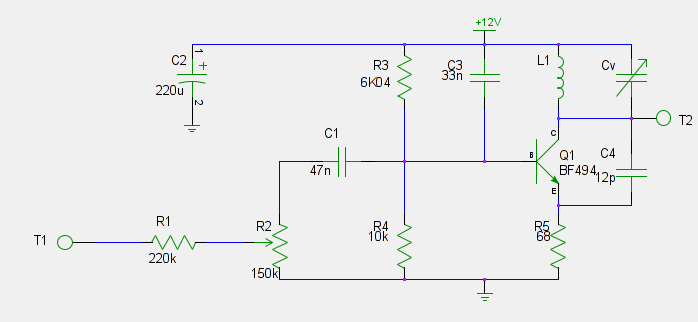
\includegraphics[scale=0.5,clip]{./imagens/FM_Modulator.png}
\end{center}
\caption{Modulador FM.}
\label{fig:modulador_FM}
\end{figure}

O sinal modulante é aplicado através do potenciômetro, que ajusta a potência do sinal entregue ao transistor $Q_1$, polarizado no ponto de operação por meio dos resistores $R_3$ e $R_4$. O tanque ressonante tem o papel de gerar a onda portadora, e sua frequência será determinada por $L_1$ e $C_v$.

Com o transistor polarizado, o sinal modulante já estabilizado será entregue à base do transistor, o sinal aparecerá novamente no coletor do mesmo, agora já modulado em frequência, pronto para ser transmitido pela antena ligada no ponto $T_2$.

\section{Demodulação de FM}
Para uma demodulação em frequência ser realizada é necessário um dispositivo que, a partir de uma onda modulada em frequência, produza um sinal de saída com amplitude diretamente proporcional à sua frequência instantânea.

A demodulação deste tipo de sinal é muito mais complexa do que a demodulação feita para os sinais em amplitude modulada. As principais estratégias para a demodulação são:
\subsection{Detector de Quadratura}
O detector de quadratura divide o sinal modulado em dois. Um os sinais passa através de um capacitor de alta reatância, assim deslocando a fase do sinal em 90 graus. Esse sinal é aplicado então a um circuito LC, cuja frequência natural de ressonância é a mesma da portadora. Se a frequência do sinal modulado em frequência for igual à da portadora, os dois sinais então terão um defasamento de 90 graus entre eles, ou seja, estarão em \textit{quadratura de fase}.

Os dois sinais são então multiplicados juntos em um dispositivo analógico ou digital que funciona como um detector de fase, isto é, um dispositivo o qual sua saída é proporcional a diferença de fase dos dois sinais.
No caso de um sinal recebido que não tenha sido modulado, a saída do detector de fase será, em média, zero. No caso de um sinal modulado, então haverá uma diferença na frequência deste sinal em relação a frequência central (frequência da portadora), neste caso o circuito LC ressonante vai deslocar a fase do sinal recebido do capacitor, sendo assim a variação total da fase do sinal serão os 90 graus impostos pelo defasamento do capacitor e mais uma variação (positiva ou negativa) imposta pelo circuito LC. A saída do detector de fase agora difere de zero, e dessa forma o sinal original usado para modular a onda da portadora pode ser recuperado.
\subsection{\textit{Phase-Locked Loop} (PLL)}
O laço de bloqueio de fase (\textit{Phase-Locked Loop}) não necessita de um circuito LC ressonante para realizar a demodulação. Ele é composto de um bloco detector ou comparador de fase, um filtro passa-baixa e um oscilador controlado por tensão (VCO - \textit{voltage controlled oscillator}). Neste sistema, o oscilador controlado por tensão tem sua fase bloqueada por um laço de realimentação negativa, forçando o VCO a seguir as variações do sinal modulado de entrada. A tensão resultante de baixa frequência que sai do filtro passa-baixa e faz com que o VCO siga a frequência do sinal de entrada é o sinal demodulado.

\subsection{Detector de Foster-Seeley}
Este circuito foi criado em 1936 por Dudley E. Foster e Stuart William Seeley visando a construção de um controle de frequência automática de receptores, porém encontrou utilidade também como demodulador de frequência. 
Ele utiliza um transformador de radiofrequência que converte variações em frequência para variações em amplitude. O transformador, sintonizado na frequência da portadora, é ligado a dois diodos retificadores, semelhante a um retificador de onda completa em ponte.
Se a frequência de entrada for a mesma da portadora, as duas metades do circuito do transformador de radiofrequência produzem a mesma queda de tensão e a saída é igual a zero. A medida que ocorrem diferenças o equilíbrio entre as duas metades do secundário do transformador varia e o resultado vem a ser uma tensão proporcional ao desvio de frequência da portadora.
Note que esse circuito é sensível a variações na amplitude, diferente de alguns detectores. Isso implica na necessidade do uso de uma etapa com um amplificador limitador antes do detector, removendo assim as variações indesejadas na amplitude as quais seriam adicionadas como ruídos.

\chapter{Item 4: Modulação por codificação de pulso (PCM)}
\section{Introdução}
\subsection{O que é modulação por codificação de pulso (PCM)?}
PCM (\textit{Pulse Code Modulation}) é um método para a representação de sinais analógicos convertidos para formato digital, visando transmissão ou posterior processamento. Uma codificação em PCM transforma uma amostra quantizada em um número codificado. \cite{renato}

A técnica consiste na quantização dos dados através de um conversor A/D. No lado do receptor existirá um conversor D/A que irá fazer o processo oposto (demodulação). Temos como vantagem o fato da qualidade do sinal recebido depender principalmente da origem, não do caminho.
\subsection{Operações executadas na modulação PCM}

\subsubsection{Amostragem da onda}
O sinal originalmente analógico é amostrado a intervalos periódicos regulares o qual captura pontos do sinal para a quantização. Neste passo se extraem amostras representativas do sinal; portanto, quanto mais amostras melhor o resultado.

É necessário que essa amostragem seja feita em uma frequência maior do que o dobro do sinal sendo amostrado (critério de Nyquist). Caso contrário a recuperação do sinal amostrado torna-se impossível.
\subsubsection{Quantização}
Neste passo cada nível é associado a um valor de bits. Aqui, devido à natureza do processo e às características dos conversores analógico/digitais, ocorrem os erros de quantização.
\subsubsection{Codificação}
Aqui gera-se o código binário propriamente dito, aplicando-se posteriores processamentos (codificações de linha, compressão digital) etc...

\begin{figure}[H]
\begin{center}
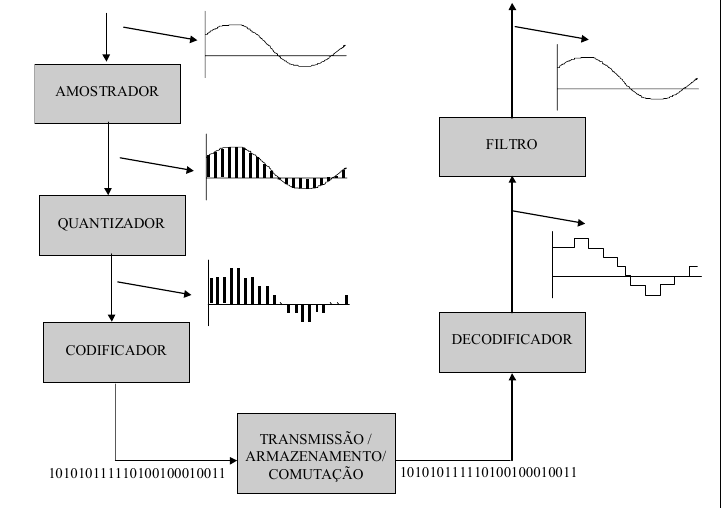
\includegraphics[scale=0.5,clip]{./imagens/etapas_PCM.png}
\end{center}
\caption{Etapas do processo de codificação PCM. \cite{moecke}}
\label{fig:pcm}
\end{figure}


\subsection{Questão prática}


Considere que a sequência de amostras [-0,15;3;1;1,8;-2;4;-3,8;4;6,5;-7;5,2]  foi extraída de um sinal analógico senoidal confinado à faixa de -8 a 8 V.

Determine:

\begin{itemize}
\item{A distância entre níveis de quantização}\newline
Para $N$ níveis = $2^n$ bits, temos que a distância entre níveis pode ser dada por

\begin{equation}
\Delta = \frac{2 A}{N}
\end{equation}


Assim, para 3 bits teremos que $\Delta = \frac{2*8}{2^3} =  2$  volts.
\item{Os níveis de quantização}

\begin{tabular}{|c|c|c|c|c|c|c|}
\hline Amostra  & Mín. intervalo  & Max. intervalo & Nível & Código  & Erro & $Erro^2$ \\ 
\hline 6,5 & 6 & 8  & 7 & 111 & -0,5 & 0,25 \\ 
\hline 5,2 & 4 & 6  & 5 & 110 & 0,2 & 0,04 \\ 
\hline 4 & 4 & 6  & 5 & 110 & -1 & 1 \\ 
\hline 4 & 4 & 6  & 5 & 110 & -1 & 1 \\ 
\hline 3 & 2 & 4 & 3  & 101  & 0 & 0 \\ 
\hline 1 & 0 & 2 & 1 & 100  &  0 & 0 \\ 
\hline 1,8 & 0 & 2 & 1 & 100 & 0,8 & 0,64 \\ 
\hline -0,15 & -2 & 0 & -1  & 011  & 0,85 & 0,7225 \\ 
\hline -2 & -4 & -2 & -3 & 010  & 1 & 1 \\ 
\hline -3,8 & -4 & -2  & -3  & 010 & -0,8 & 0,64 \\ 
\hline -7 & -8 & -6  &  -7 & 000  & 0 & 0 \\ 
\hline 
\end{tabular} 

Níveis: -7, -5, -3, -1, 1, 3, 5, 7.
\item{O erro médio quadrático de quantização}

Sendo o erro calculado tirando-se a amostra menos o nível em que ela se encontra. O erro médio quadrático será o somatório dos erros elevados ao quadrado e divididos pelo número de amostras.

Obtém-se um valor de $e = 0,481136$.

\item{Relação sinal/ruído considerando uma carga de 1 $\Omega$}

A relação sinal-ruído é de $SNR = S/e^2$, sendo que S é a potência média deste sinal, dado pela resistência de 1 $\Omega$.

O erro médio $e$ de quantização é dado por \cite{renato}

\begin{equation}\label{emq}
\epsilon = \frac{1}{\Delta}\int\limits_{-\Delta/2}^{\Delta/2} \epsilon^2 d\epsilon = \frac{\Delta^2}{12}
\end{equation}

Como $\Delta = \frac{2 A}{N}$, substituindo-se em \ref{emq}  tem-se que
\begin{equation}\label{epsilonnovo}
\epsilon = \frac{A^2}{3N^2}
\end{equation}

Para o SNR temos a expressão

\begin{equation}\label{snrdb}
SNR_{db} = 10 \log{\frac{S}{\epsilon^2}}
\end{equation}

substituindo-se \ref{epsilonnovo} temos

\begin{displaymath}
SNR_{db} = 10 \log(\frac{3 N^2}{2}) 
\end{displaymath}

\begin{displaymath}
SNR_{db} = 10 \log(\frac{3}{2}) + 20 \log(N) \newline
\end{displaymath}W

\begin{displaymath}
SNR_{db}=1,76 + 20 \log(2^b) \newline
\end{displaymath}

por fim chegando-se a:
\begin{equation}
SNR_{db}=1,76 + 6,02 b
\end{equation}

Para 3 bits ($b=3$) obtém-se que esse valor será de \textbf{19,82 dB}.

\item{A sequência PCM a ser transmitida}

A sequência a ser transmitida será de \texttt{[011 101 100 100 010 110 010 110 111 000 110]}.

\end{itemize}
\chapter{Conclusão}
Modulações analógicas, como as vistas neste trabalho, continuam sendo importantes devido à sua simplicidade e baixo custo de implementação; assim, é provável que sejam usadas por muito tempo. Já a codificação PCM, abordada de forma teórica, é amplamente empregada em sistemas computacionais e de transmissão digital de dados.

Os experimentos realizados em laboratório foram relevantes, possibilitando-nos a visualização e interpretação do comportamento dos circuitos de modulação.

\bibliographystyle{alpha}
\begin{thebibliography}{100}
\bibitem{renato}
 MACHADO, R. 
 \textbf{Notas de aula da disciplina de Comunicação de Dados.}
 Disponível em \url{http://www.ufsm.br/gpscom/professores/Renato\%20Machado/comunicacaodedados.html}. Acessado em 12/06/2012.
 
\bibitem{lamar}
LAMAR, V. M. \textbf{Modulação em Amplitude}. Disponível em \url{http://www.cic.unb.br/~lamar/te060/Apostila/Capitulo2.pdf}. Acesso em 23/06/2012.

 
\bibitem{BF494}
\textbf{BF494, BF495 NPN Medium-Frequency Transistors}. Disponível em \url{http://www.datasheetcatalog.org/datasheet/philips/BF494B.pdf}. Acesso em 23/06/2012.

\bibitem{teleco}
\textbf{O Início da Digitalização - Telefonia Fixa}. Disponível em \url{http://www.teleco.com.br/tutoriais/tutorialciclos/pagina_4.asp}. Acesso em 27/06/2012.

\bibitem{campos}
\textbf{Modulação e Demodulação de Sinal}. Disponível em \url{http://www.del.ufms.br/PCI_T1/G6/Modulacao.htm}. Acesso em 28/06/2012.

\bibitem{medeiros}
MEDEIROS, M. C.. \textbf{Comunicações Digitais}. Disponível em \url{http://intranet.deei.fct.ualg.pt/archive/SCom_2005_2006/}. Acesso em 01/07/2012.

\bibitem{moecke}
MOECKE, M. \textbf{Modulação por Código de Pulso}. Disponível em \url{http://manoel.pesqueira.ifpe.edu.br/fmn/anterior/2008.1/Telefonia/Mod_PCM.pdf}. Acesso em 03/07/2012.
\end{thebibliography}
\end{document}          
